\documentclass[a4paper]{article}
\usepackage{graphicx}
\usepackage{amsmath}
\usepackage{xr}


\usepackage[round]{natbib}
\bibliographystyle{plainnat}

\usepackage{lineno}
\usepackage{xcolor}

\externaldocument[main-]{main}
\renewcommand{\thefigure}{S\arabic{figure}}

\allowdisplaybreaks

\begin{document}

\title{Supp. Info. for ``Process-based modelling of microbial community dynamics in the human colon''}

\author{Helen Kettle, Petra Louis and Harry J. FLint}

\maketitle

\linenumbers

\section{Mathematical Model}
\subsection{Simple Model}
In this section we present a very simple model with one microbial group and one colon compartment that we then use to derive bounds on parameters (e.g. absorption of SCFA and water) and to look at the bulk properties of the system, e.g. the relationship between transit time and SCFA concentration.

This simple model consists of, bacteria ($X$), substrate ($S$), SCFA mass ($Z$) and water ($W$) all with units of mass. We set $f_s$ as the fraction of the waste products of $X$ that are SCFA, and $Y$ is the amount of microbial growth for 1 g of $S$ and $a_Z$ and $a_W$ are the absorption rates of $Z$ and $W$.
The rates of change are given by
\begin{eqnarray}
\frac{dX(t)}{dt}&=&G(t)X(t)-X(t)V\\\label{eq:TtSSB}
\frac{dS(t)}{dt}&=&\dot{S_{in}}-\frac{G(t)X(t)}{Y}-S(t)V\\
\frac{dZ(t)}{dt}&=&f_s\left(\frac{1}{Y}-1\right)G(t)X(t)-(V+a_Z)Z(t)\\
\frac{dW(t)}{dt}&=&\dot{W_{in}}-(V+a_W)W(t)\label{eq:TtSSW}
\end{eqnarray}
where microbial growth, $G$, is given by
\begin{equation}
G(t)=G^m\frac{S(t)}{S(t)+K}
\end{equation}
where $K$ is the half-saturation constant and $G^m$ is the maximum growth rate of $X$ on $S$.
Transit time is incorporated via the washout rate, $V$ such that $V=1/T_t$.

Steady state analysis (i.e. when the system is not changing with time) of the one group model can be used to give us some bounds or checks on the bulk properties of the system. 
The steady state solution (at time, $t_s$), assuming $X>0$, is given by 
%\textcolor{red}{[/R/transitTimeModel.R]} 
\begin{eqnarray}
%V&=&G(P,S,W)\\
X(t_s)&=&(\dot{S_{in}}/V-S(t_s))Y\\
S(t_s)&=&\frac{VK}{G^{\max}-V}\\
Z(t_s)&\approx & VX(t_s)\frac{1-Y}{Y(a_Z+V)}\\
W(t_s)&=&\frac{\dot{W_{in}}}{a_W+V}\label{eq:Wss1}
\end{eqnarray}
where $\dot{X_{in}}$ is the inflow rate of $X$.

\subsection{Microbial yield and substrate inflow}
Assuming the microbes consume all available substrate, then the steady state mass of microbes can be approximated by 
\begin{equation}
X(t_s) \approx \frac{\dot{S_{in}}Y}{V}\label{eq:Xss}
\end{equation}
where $\dot{S}_{in}$ is the dietary inflow of all substrates (i.e. dietary P, C and mucin); $V$ is the wash out rate from the system and $Y$, the microbial yield.
Assuming the output of microbes (given by $X_{t_s}V$) is 14-28 g d$^{-1}$ \citep{StephenCummings} (with midpoint of 21) and the substrate inflow is about 65 g d$^{-1}$; Eq. \ref{eq:Xss} suggests that $Y$ is 21/65 i.e. about 0.3 which matches very well with the yield values for our functional groups which have yield values around 0.28 or 0.33 (see other Supp. Info. file).

\subsection{Specific water absorption, $a_W$}
Extending Eq. \ref{eq:Wss1} to $N$ compartments with downstream flow from 1 to N, and assuming the specific absorption rate is the same in all, then at steady state the water in each compartment is given by,
\begin{eqnarray}
    W_1&=&\frac{\dot{W}_{in}}{a_W+V_1},\\
    W_2&=&\frac{W_1V_1}{a_W+V_2},...\\
    ..., W_N&=&\frac{W_{N-1}V_{N-1}}{a_W+V_N}
\end{eqnarray}
Successively substituting for the unknowns gives 
\begin{equation}
    W_N=\frac{\dot{W}_{in}V_1V2...V_{N-1}}{(a_W+V_1)(a_W+V_2)...(a_W+V_N)}
    \label{eq:Wn}
\end{equation}
If 90\% of water is absorbed over the transit time then in the last compartment, $N$, $W_NV_N=0.1\dot{W}_{in}$. Substituting this into Eq. \ref{eq:Wn} gives
\begin{equation}
    \prod_{k=1}^N(a_W+V_k)=10\prod_{j=1}^NV_j.
\end{equation}
This can be solved numerically where $V_j$ is computed by dividing the colon into $N$ compartments which each take fraction, $f^T_j$, of the total transit time to pass through. Using fractional times based on compartment volume (Fig. 1 in main manuscript) and assuming that $a_W$ is the same in each compartment we find that for a one compartment model, $a_W=\frac{9}{T_t}$; for a two compartment model, $a_W=\frac{4.59}{T_t}$; and for a three compartment model, $a_W=\frac{3.72}{T_t}$ (see Fig. \ref{fig:aWaZ}). This can be expressed exactly by
\begin{equation}
    a_W=\frac{16.95-9.72N+1.77N^2}{T_t}\label{eq:aW}
\end{equation}
where $N$ is the number of compartments in the model. Note that this does not mean that specific water absorption changes with transit time, rather that to fulfill the 90\% absorption criteria we can set $a_W$ based on $N$ and $T_t$. 
Once a typical transit time is chosen, the value of $a_W$ can be fixed.
As a rough estimation, $a_W\approx 3$ /d for a 3 compartment model with a transit time between one to one and a half days (Fig. \ref{fig:aWaZ}).
Given this will not be significantly affected by the microbial model (microbial uptake/production of water is small) this result will apply to all of the models in this work.

%findaW.R

\begin{figure}
    \centering
    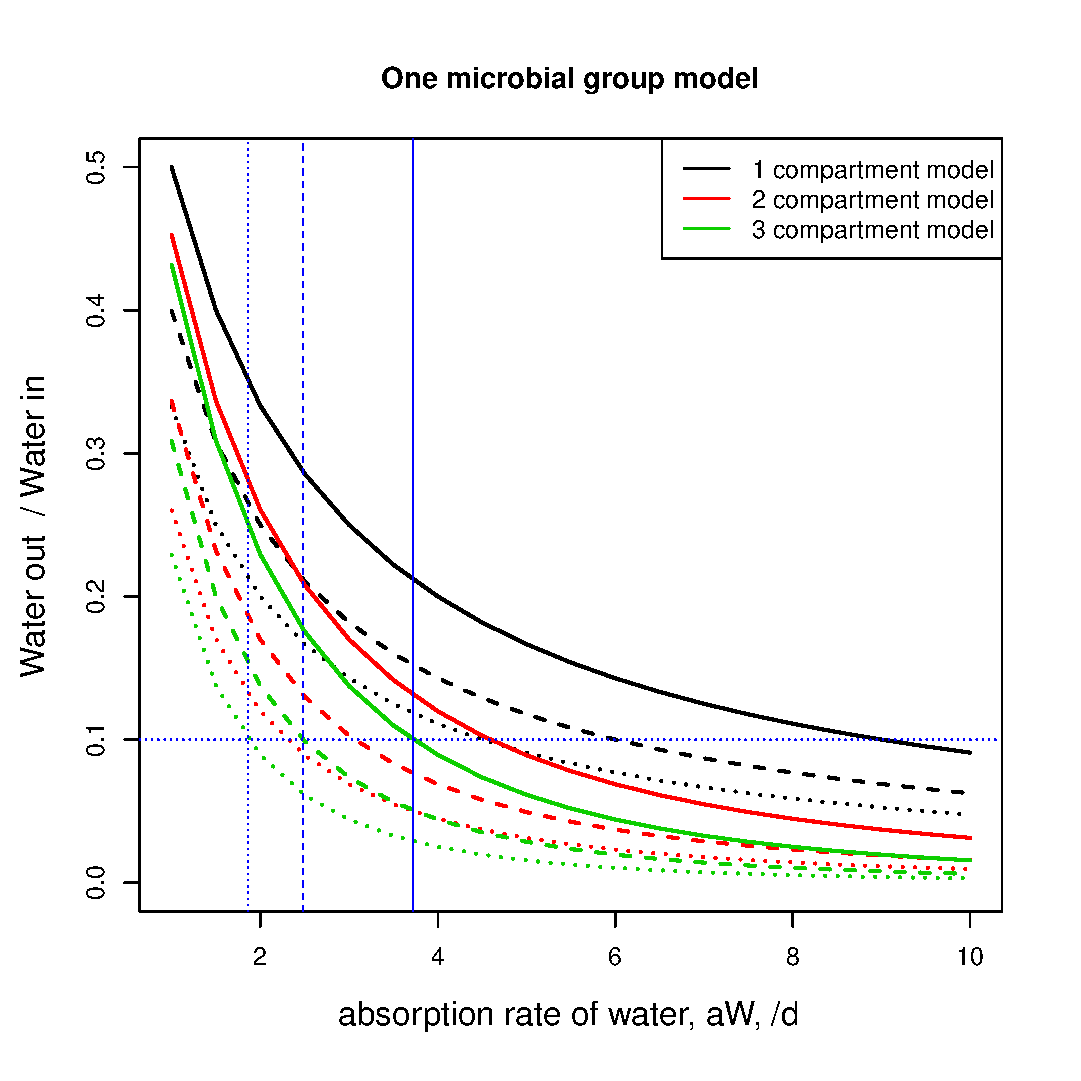
\includegraphics[scale=0.32]{images/aW.eps}
    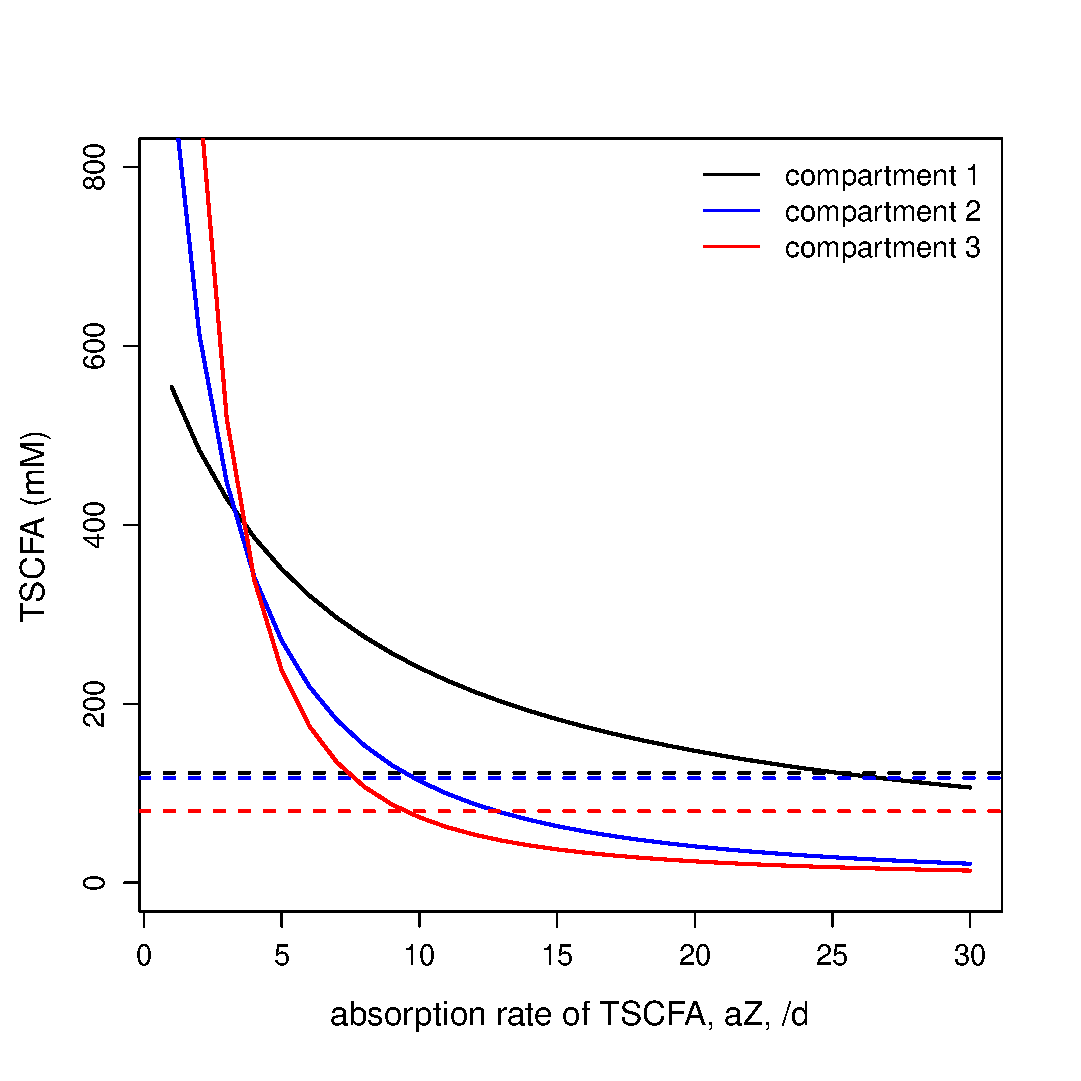
\includegraphics[scale=0.32]{images/aZconstant.eps}
    \caption{a) Achieving 90\% water absorption for different transit times (1, 1.5 and 2 days represented by solid, dashed and dotted line respectively) and different number of compartments (1, 2, and 3 by colour, as shown in legend). The dotted horizontal line shows the required value for 90\% incoming water absorption in the colon and the vertical blue lines show the $a_W$ value which gives the correct total absorption for the 3 different transit times (which are as before, 1, 1.5 and 2 days represented by solid, dashed and dotted line respectively). 
%[plotOneGroup.R]
    b) Investigating SCFA absorption. TSCFA (mM) for different $a_Z$ for transit time of 1.25 days, for the one group, three compartment model. $a_Z$ is from 1,2,...30 /d with values constant throughout the colon. The dashed horizontal lines show the expected TSCFA in each compartment. The simulation is for 5 days and the results are the mean over the last day. Constant inflow and outflow (no meals or bowel movements) with $a_W$ changing with transit time according to Eq. \ref{eq:aW}. 
%[plotOneGroup.R]
    }
    \label{fig:aWaZ}
\end{figure}




\subsection{Specific SCFA absorption, $a_Z$}

Using our one group microbial group model but adapted for 3 compartments, and our estimation for $a_W$ based on transit time and the number of compartments (Eq. \ref{eq:aW}), we run the model for a transit times of 1.25 d with continuous inflow and outflow, over a range of $a_Z$ from 1-30 d$^{-1}$.
We compute TSCFA from our model by converting $Z$ from g to mM  using 
\begin{equation}
    Z_{mM}=10^6\frac{Z_g}{W_g m_Z}
\end{equation}
where $m_Z$ is computed by assuming TSCFA is in the ratio 3:1:1 (Ac:Bu:Pr) to give a weighted mean molar mass of TSCFA, $m_Z$ of 68.4 g mol$^{-1}$.
Fig. \ref{fig:aWaZ}, shows the TSCFA in each model compartment versus $a_Z$. The horizontal dashed lines show the TSCFA value matching the model criteria, indicating the best estimates were $a_Z$ equal to 25.2, 4.2 and 9.2 d$^{-1}$ in the proximal, transverse and distal colon respectively.
However, this was determined using $a_Z$ constant through the colon so if $a_Z$ varies between compartments this will change the results. 
In the interests of a robust model (i.e. the fewer parameter values, the better) we made the decision to use one value for $a_Z$ . 
Given the experimental value of 9.6 d$^{-1}$ compares well with our best estimate for the distal colon (9.2 $d^{-1}$) we decided to set aZ =9.6 d$^{-1}$ throughout. 
It should be noted however that decreasing $a_Z$ along the colon has been implemented in other models e.g. \cite{Labarthe}. 






\section{Effect of Transit Time}
Experimental evidence (e.g. \citep{Lewis}) shows that TSCFA (mM) decreases as transit time increases. We can explain why this is, mathematically, using a very simple one group model with monod growth, which we can solve analytically at steady state.
To compute TSCFA in mM we need to use the fraction of $P$ that is SCFA and then divide by the mean molor mass ($m_m$)and multiply by 1000 to find mmol. We then need to divide by $W$ in litres, thus,
\begin{equation}
\mbox{TSCFA}=10^6\frac{Pf_s}{W m_m}
\end{equation}
Substituting for $P$ and $W$, ignoring scaling constants and assuming remaining substrate at steady state is negligible, shows that TSCFA is linearly related to the expression
\begin{equation}
\frac{\dot{S_{in}}}{\dot{W_{in}}}\frac{a_W+V}{a_P+V}
\end{equation}
To see the effect of simply changing the transit time through the colon on TSCFA we assume $\dot{S_{in}}$ and $\dot{W_{in}}$ are fixed and replace $V$ by $1/Tt$ to get
\begin{equation}
TSCFA \propto \frac{a_WT_t+1}{a_PT_t+1}
\end{equation}
Since we have $a_W$=3 and $a_P$=9.6, the denominator will increase much faster than the numerator as $T_t$ increases thus, theoretically, TSCFA will decrease as transit time increases as SCFA are absorbed faster than water.
Using realistic parameter values in the above model (Eq. \ref{eq:TtSSB}-\ref{eq:TtSSW}) allows us to plot TSCFA against transit time  -- see Fig \ref{fig:transitTimeAnal} which compares very well with the experimental data shown in Fig. 1 by \citet{Lewis}.

\begin{figure}
    \centering
    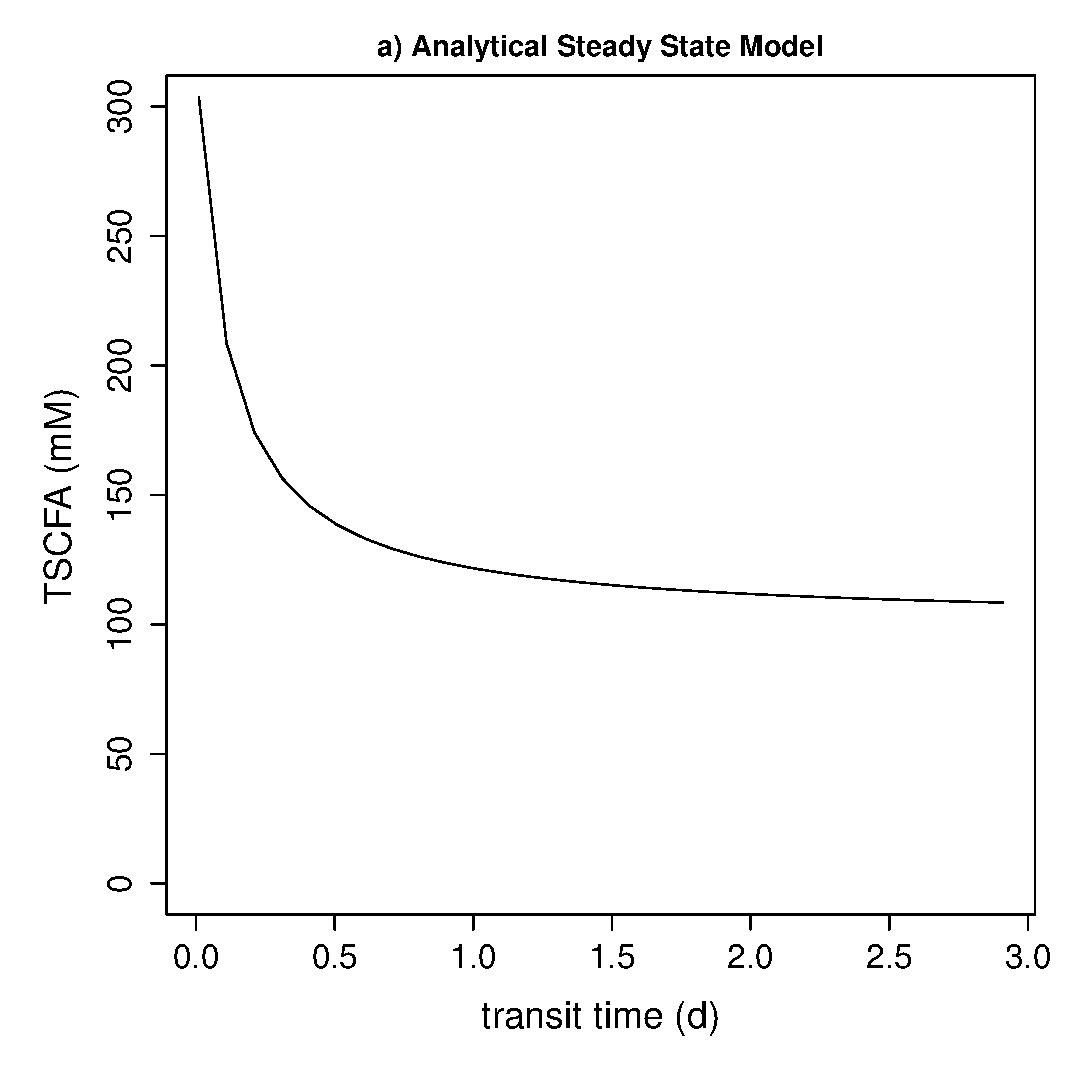
\includegraphics[scale=0.4]{images/TSCFAandTt.eps}
    \caption{TSCFA as a function of transit time obtained from the solution of Eqs. \ref{eq:TtSSB}-\ref{eq:TtSSW}. We convert from product mass, $P$, to moles using the average molar mass (weighted according to A:B:P = 3:1:1) of 68.5 g/mol and compute $f_s$ as an average of the microPop microbial group stoichiometries to be approximately 0.5. We set inflowing substrate at 65 g/d (dietary substrate plus mucin) and inflowing water at 1100 g/d, with parameter values $Y$=0.3, $G^{\max}$=20 /d and $K$=0.001. [transitTimeModel.R]
    }
    \label{fig:transitTimeAnal}
\end{figure}


\section{Microbial group parameter values}
The parameters describing the different microbial groups are the same as the intrinsic functional groups given in the microPop R package (version 1.6), with one exception. We increased the maximum growth rate of Lactate Producers on RS from 6  d$^{-1}$ to 7  d$^{-1}$ and their pH tolerance were cordinates changed to tolerate lower pH (first two pH coordinates now 4.5 and 5.25, rather than 4.95 and 5.7) to ensure a better chance of their survival in the model. 
This section shows the data frames used for each microbial group in microPopGut. The following list explains the different entries in these data frames.
\begin{itemize}
\item `Rtype' refers to the substrate type on the pathway:
\begin{itemize}
\item `X': not involved in pathway
\item `S': substitutable substrate (this can be interchanged with other substitutable substrates)
\item `Se': essential substrate (the microbes can not grow without this)
\item `Sb': boosting substrate (if this is present the microbe can grow faster) 
\item `Sw': water
\item `P': metabolic product
\end{itemize}
\item `halfsat' is the half saturation constant for monod growth
\item `yield' is the microbial mass produced from one gram of substrate
\item `maxGrowthRate' is the specific maximum growth rate of the microbes 
\item `stoichiom' refers to the number of moles of each molecules involved in growth
\item `keyResource' is the substrate whose uptake rate is used to compute the uptake of the other substrates on the pathway according to the stoichiometry
\item `numPathways' defines how many metabolic pathways the microbial group has. 
When there is more than one pathway, numbered parameter names for the subsequent pathways are used.
\end{itemize}
For more details please refer to \cite{Kettle2015} and \cite{Kettle2018} or use the help function within the microPopGut package.



\begin{table}[ht]
\caption{Bacteroides} 
\centering
\resizebox{\textwidth}{!}{ %add this
\begin{tabular}{rllllllllll}
  \hline
 & units & Protein & NSP & RS & Acetate & Propionate & Succinate & H2 & CO2 & other \\ 
  \hline
Rtype & none & X & S & S & P & P & P & P & P & X \\ 
  halfSat & g/l &  & 0.001 & 0.001 &  &  &  &  &  &  \\ 
  yield & g/g &  & 0.286 & 0.333 &  &  &  &  &  &  \\ 
  maxGrowthRate & /d &  & 12 & 24 &  &  &  &  &  &  \\ 
  stoichiom & mol &  & 2 & 2 & 2 & 1 & 1 & 2 & 1 &  \\ 
  keyResource & none &  &  &  &  &  &  &  &  &  \\ 
  numPathways & none & 2 &  &  &  &  &  &  &  &  \\ 
  \hline
  Rtype.2 & none & S & X & X & P & P & P & P & P & P \\ 
  halfSat.2 & g/l & 0.001 &  &  &  &  &  &  &  &  \\ 
  yield.2 & g/g & 0.2 &  &  &  &  &  &  &  &  \\ 
  maxGrowthRate.2 & /d & 24 &  &  &  &  &  &  &  &  \\ 
  stoichiom.2 & mol & 6 &  &  & 2 & 1 & 1 & 2 & 1 & 7 \\ 
  keyResource.2 & none &  &  &  &  &  &  &  &  &  \\ 
  \hline
  pHcorners & pH & 5.6 & 6.35 & 7.85 & 8.6 &  &  &  &  &  \\ 
  \hline
\end{tabular}}
\end{table}


\begin{table}[ht]
\caption{NoButyStarchDeg} 
\centering
\resizebox{\textwidth}{!}{ %add this
\begin{tabular}{rlllllll}
  \hline
 & units & NSP & RS & Acetate & H2 & CO2 & H2O \\ 
  \hline
Rtype & none & S & S & P & P & P & Sw \\ 
  halfSat & g/l & 0.001 & 0.001 &  &  &  &  \\ 
  yield & g/g & 0.286 & 0.333 &  &  &  &  \\ 
  maxGrowthRate & /d & 3.6 & 14.4 &  &  &  &  \\ 
  stoichiom & mol & 1 & 1 & 2 & 4 & 2 & 2 \\ 
  keyResource & none &  &  &  &  &  &  \\ 
  numPathways & none & 1 &  &  &  &  &  \\ 
  \hline
  pHcorners & pH & 5.35 & 6.1 & 7.6 & 8.35 &  &  \\ 
  \hline
\end{tabular}}
\end{table}

% latex table generated in R 3.6.0 by xtable 1.8-4 package
% Thu Jun  2 12:48:16 2022
\begin{table}[ht]
\caption{NoButyFibreDeg} 
\centering
\resizebox{\textwidth}{!}{ %add this
\begin{tabular}{rllllll}
  \hline
 & units & NSP & RS & Acetate & Succinate & H2 \\ 
  \hline
Rtype & none & S & S & P & P & P \\ 
  halfSat & g/l & 0.001 & 0.001 &  &  &  \\ 
  yield & g/g & 0.286 & 0.333 &  &  &  \\ 
  maxGrowthRate & /d & 16.8 & 3.6 &  &  &  \\ 
  stoichiom & mol & 1 & 1 & 1 & 1 & 1 \\ 
  keyResource & none &  &  &  &  &  \\ 
  numPathways & none & 1 &  &  &  &  \\ 
  \hline
  pHcorners & pH & 5 & 5.75 & 7.25 & 8 &  \\ 
  \hline
\end{tabular}}
\end{table}
% latex table generated in R 3.6.0 by xtable 1.8-4 package
% Thu Jun  2 12:48:16 2022
\begin{table}[ht]
\centering
\caption{LactateProducers} 
\resizebox{\textwidth}{!}{ %add this
\begin{tabular}{rlllllllll}
  \hline
 & units & NSP & RS & Sugars & Acetate & Lactate & Formate & Ethanol & H2O \\ 
  \hline
Rtype & none & S & S & S & P & P & P & P & Sw \\ 
  halfSat & g/l & 0.001 & 0.001 & 0.001 &  &  &  &  &  \\ 
  yield & g/g & 0.286 & 0.333 & 0.333 &  &  &  &  &  \\ 
  maxGrowthRate & /d & 7.2 & 7 & 24 &  &  &  &  &  \\ 
  stoichiom & mol & 6 & 6 & 6 & 10 & 4 & 2 & 1 & 1 \\ 
  keyResource & none &  &  &  &  &  &  &  &  \\ 
  numPathways & none & 1 &  &  &  &  &  &  &  \\ 
  \hline
  pHcorners & pH & 4.5 & 5.25 & 7.2 & 7.95 &  &  &  &  \\ 
  \hline
\end{tabular}}
\end{table}
% latex table generated in R 3.6.0 by xtable 1.8-4 package
% Thu Jun  2 12:48:16 2022
\begin{table}[ht]
\caption{ButyrateProducers1} 
\centering
\resizebox{\textwidth}{!}{ %add this
\begin{tabular}{rlllllllll}
  \hline
 & units & NSP & RS & Sugars & Acetate & Butyrate & H2 & CO2 & H2O \\ 
  \hline
Rtype & none & S & S & S & Sb & P & P & P & P \\ 
  halfSat & g/l & 0.001 & 0.001 & 0.001 & 0.001 &  &  &  &  \\ 
  yield & g/g & 0.286 & 0.333 & 0.333 &  &  &  &  &  \\ 
  maxGrowthRate & /d & 8.4 & 8.4 & 24 &  &  &  &  &  \\ 
  stoichiom & mol & 2 & 2 & 2 & 2 & 3 & 2 & 4 & 2 \\ 
  keyResource & none & Hex &  &  &  &  &  &  &  \\ 
  numPathways & none & 1 &  &  &  &  &  &  &  \\ 
  nonBoostFrac & none & 0.75 &  &  &  &  &  &  &  \\ 
  \hline
  pHcorners & pH & 4.95 & 5.7 & 7.2 & 7.95 &  &  &  &  \\ 
  \hline
\end{tabular}}
\end{table}
% latex table generated in R 3.6.0 by xtable 1.8-4 package
% Thu Jun  2 12:48:16 2022
\begin{table}[ht]
\caption{ButyrateProducers2} 
\centering
\resizebox{\textwidth}{!}{ %add this
\begin{tabular}{rllllllllll}
  \hline
 & units & NSP & RS & Sugars & Acetate & Butyrate & Lactate & Formate & CO2 & H2O \\ 
  \hline
Rtype & none & S & S & S & Sb & P & P & P & P & P \\ 
  halfSat & g/l & 0.001 & 0.001 & 0.001 & 0.001 &  &  &  &  &  \\ 
  yield & g/g & 0.286 & 0.333 & 0.333 &  &  &  &  &  &  \\ 
  maxGrowthRate & /d & 14.4 & 7.2 & 24 &  &  &  &  &  &  \\ 
  stoichiom & mol & 6 & 6 & 6 & 4 & 7 & 2 & 6 & 4 & 4 \\ 
  nonBoostFrac & none & 0.1 &  &  &  &  &  &  &  &  \\ 
  keyResource & none & Hex &  &  &  &  &  &  &  &  \\ 
  numPathways & none & 1 &  &  &  &  &  &  &  &  \\ 
  pHcorners & pH & 4.85 & 5.6 & 7.1 & 7.85 &  &  &  &  &  \\ 
   \hline
\end{tabular}}
\end{table}
% latex table generated in R 3.6.0 by xtable 1.8-4 package
% Thu Jun  2 12:48:16 2022
\begin{table}[ht]
\caption{PropionateProducers} 
\centering
\resizebox{\textwidth}{!}{ %add this
\begin{tabular}{rlllllllll}
  \hline
 & units & NSP & RS & Sugars & Acetate & Propionate & CO2 & Lactate & H2O \\ 
  \hline
Rtype & none & S & S & S & P & P & P & X & P \\ 
  halfSat & g/l & 0.001 & 0.001 & 0.001 &  &  &  &  &  \\ 
  yield & g/g & 0.286 & 0.333 & 0.333 &  &  &  &  &  \\ 
  maxGrowthRate & /d & 7.2 & 7.2 & 24 &  &  &  &  &  \\ 
  stoichiom & moles & 3 & 3 & 3 & 2 & 4 & 2 &  & 2 \\ 
  keyResource & none &  &  &  &  &  &  &  &  \\ 
  numPathways & none & 2 &  &  &  &  &  &  &  \\ 
  \hline
  Rtype.2 & none & X & X & X & P & P & P & Se & P \\ 
  halfSat.2 & g/l &  &  &  &  &  &  & 0.001 &  \\ 
  yield.2 & g/g &  &  &  &  &  &  & 0.111 &  \\ 
  maxGrowthRate.2 & /d &  &  &  &  &  &  & 4.8 &  \\ 
  stoichiom.2 & moles &  &  &  & 1 & 2 & 1 & 3 & 1 \\ 
  keyResource.2 & none & Lactate &  &  &  &  &  &  &  \\ 
  \hline
  pHcorners & pH & 4.75 & 5.5 & 7 & 7.75 &  &  &  &  \\ 
  \hline
\end{tabular}}
\end{table}
% latex table generated in R 3.6.0 by xtable 1.8-4 package
% Thu Jun  2 12:48:16 2022
\begin{table}[ht]
\caption{ButyrateProducers3} 
\centering
\resizebox{\textwidth}{!}{ %add this
\begin{tabular}{rlllllllllll}
  \hline
 & units & NSP & RS & Sugars & Acetate & Butyrate & Formate & H2 & CO2 & Lactate & H2O \\ 
  \hline
Rtype & none & S & S & S & P & P & P & P & P & X & Sw \\ 
  halfSat & g/l & 0.001 & 0.001 & 0.001 &  &  &  &  &  &  &  \\ 
  yield & g/g & 0.286 & 0.333 & 0.333 &  &  &  &  &  &  &  \\ 
  maxGrowthRate & /d & 7.2 & 7.2 & 24 &  &  &  &  &  &  &  \\ 
  stoichiom & mol & 10 & 10 & 10 & 2 & 9 & 12 & 10 & 8 &  & 2 \\ 
  keyResource & none &  &  &  &  &  &  &  &  &  &  \\ 
  numPathways & none & 2 &  &  &  &  &  &  &  &  &  \\ 
\hline
  Rtype.2 & none & X & X & X & Se & P & X & P & P & Se & P \\ 
  halfSat.2 & g/l &  &  &  & 0.001 &  &  &  &  & 0.001 &  \\ 
  yield.2 & g/g &  &  &  &  &  &  &  &  & 0.111 &  \\ 
  maxGrowthRate.2 & /d &  &  &  &  &  &  &  &  & 4.8 &  \\ 
  stoichiom.2 & mol &  &  &  & 2 & 3 &  & 2 & 4 & 4 & 2 \\ 
  keyResource.2 & none & Lactate &  &  &  &  &  &  &  &  &  \\ 
\hline
  pHcorners & pH & 4.85 & 5.6 & 7.1 & 7.85 &  &  &  &  &  &  \\ 
   \hline
\end{tabular}}
\end{table}
% latex table generated in R 3.6.0 by xtable 1.8-4 package
% Thu Jun  2 12:48:16 2022
\begin{table}[ht]
\caption{Acetogens} 
\centering
\resizebox{\textwidth}{!}{ %add this
\begin{tabular}{rlllllllll}
  \hline
 & units & NSP & RS & Sugars & Acetate & H2 & CO2 & Formate & H2O \\ 
  \hline
Rtype & none & S & S & S & P & X & X & X & X \\ 
  halfSat & g/l & 0.001 & 0.001 & 0.001 &  &  &  &  &  \\ 
  yield & g/g & 0.286 & 0.333 & 0.333 &  &  &  &  &  \\ 
  maxGrowthRate & /d & 7.2 & 7.2 & 24 &  &  &  &  &  \\ 
  stoichiom & moles & 1 & 1 & 1 & 3 &  &  &  &  \\ 
  keyResource & none &  &  &  &  &  &  &  &  \\ 
  numPathways & none & 3 &  &  &  &  &  &  &  \\ 
\hline
  Rtype.2 & none & X & X & X & P & Se & Se & X & P \\ 
  halfSat.2 & g/l &  &  &  &  & 0.001 & 0.001 &  &  \\ 
  yield.2 & g/g &  &  &  &  &  & 0.03 &  &  \\ 
  maxGrowthRate.2 & /d &  &  &  &  &  & 2.4 &  &  \\ 
  stoichiom.2 & moles &  &  &  & 1 & 4 & 2 &  & 2 \\ 
  keyResource.2 & none & CO2 &  &  &  &  &  &  &  \\ 
\hline
  Rtype.3 & none & S & S & S & P & P & P & Se & X \\ 
  halfSat.3 & g/l & 0.001 & 0.001 & 0.001 &  &  &  & 0.001 &  \\ 
  yield.3 & g/g & 0.286 & 0.333 & 0.333 &  &  &  &  &  \\ 
  maxGrowthRate.3 & /d & 7.2 & 7.2 & 24 &  &  &  &  &  \\ 
  stoichiom.3 & moles & 1 & 1 & 1 & 3 & 2 & 2 & 2 &  \\ 
  keyResource.3 & none & Hex &  &  &  &  &  &  &  \\ 
\hline
  pHcorners & pH & 5.25 & 6 & 7.5 & 8.25 &  &  &  &  \\ 
   \hline
\end{tabular}}
\end{table}
% latex table generated in R 3.6.0 by xtable 1.8-4 package
% Thu Jun  2 12:48:16 2022
\begin{table}[ht]
\caption{Methanogens} 
\centering
\resizebox{\textwidth}{!}{ %add this
\begin{tabular}{rllllll}
  \hline
 & units & H2 & CO2 & CH4 & H2O & Formate \\ 
  \hline
Rtype & none & Se & Se & P & P & X \\ 
  halfSat & g/l & 0.001 & 0.001 &  &  &  \\ 
  yield & g/g &  & 0.03 &  &  &  \\ 
  maxGrowthRate & /d &  & 2.4 &  &  &  \\ 
  stoichiom & mol & 4 & 1 & 1 & 2 &  \\ 
  keyResource & none & CO2 &  &  &  &  \\ 
  numPathways & none & 2 &  &  &  &  \\ 
\hline
  Rtype.2 & none & X & P & P & P & Se \\ 
  halfSat.2 & g/l &  &  &  &  & 0.001 \\ 
  yield.2 & g/g &  &  &  &  & 0.00724 \\ 
  maxGrowthRate.2 & /d &  &  &  &  & 2.4 \\ 
  stoichiom.2 & mol &  & 3 & 1 & 2 & 4 \\ 
  keyResource.2 & none & Formate &  &  &  &  \\ 
  \hline
  pHcorners & pH & 5.25 & 6 & 7.5 & 8.25 &  \\ 
  \hline
\end{tabular}}
\end{table}

\clearpage

\bibliography{../refs} 

\end{document}

